% !TEX root = ../sethomas_thesis_main.tex

\section{Kirigami inspired Compliant SMA Actuators}
Using topology optimization, various compliant SMA actuators can be designed with the intent to combine the functions of the kinematic stage and the active element. However, due to the current limitations of fabrication and its costs, the feasibility of such an actuator, in the current sense, is unlikely. As additive manufacturing of SMAs becomes more accessible, the advantages of designing compliant SMA structures such as increasing the overall work density of the actuator, will become more apparent and attractive.

Kirigami, the Japanese art of cutting paper to create intricate structure, has gained traction in various engineering fields to create stretchable structure as shown in the work by \todocite. While designing 3D compliant structure made of SMA is expensive, this kirigami approach can be extended to SMAs to create compliant structures that when cut in a specific manner, can exhibit surprising mechanical behaviours.

When designing actuators, a key detail to keep in mind is the life cycle of the device. In common industrial applications, the number of cycles to fatigue of traditional grippers can exceed $10^6$ cycles. In the case of SMA actuators, this number is much lower and is directly related to the structural fatigue of the material. The determining factors regarding the fatigue life of SMAs are the strain amplitude and the type of strain applied to the material. The work by \cite{runcimanEquivalentStrainCoffin2011} looks at the fatigue lifetime of NiTiNOL based on different loading conditions, such as torsion, tension and bending. They conclude that SMAs tend to have a much longer life cycle when loading under torsion or bending when compared to tension. The results show that with a fixed strain amplitude of 1\%, in tension, the number of cycles to failure is less than $10^3$ whereas in bending or torsion, the number of cycles to failure is around $10^5$.

The availability of NiTiNOL in different geometries such as springs, wires and sheets, has allowed the creation of multiple classes of SMA actuators that exploit their respective advantages. As mentioned in previous sections, the simplest approach would be to use the alloy in the shape of a wire paired with a biasing spring to drive an actuator where the stress and strain of the material corresponds directly to the stroke and force output of the actuator. In these cases, SMA wires are elongated under pure traction and are then heated to recover the strain and provide the force output as shown in the works by \cite{kyungDesignMicrogripperMicromanipulation2008}, \cite{welschVacuumGripperSystem2018}, \cite{haibinModelingGraspingForce2018}, and \cite{andrianesisDevelopmentControlMultifunctional2015}. Here, the stroke of the actuator can not exceed 1\% without compromising its fatigue life. Thus, in cases where a larger stroke is required, the geometry of the wire is adapted to form a spring which can provide stroke above 100\% as implemented in the works by \cite{ikutaMicroMiniatureShape1990} and \cite{zhakypovOrigamiInspiredReconfigurableSuction2018}. Here, the material no longer deforms in traction but rather in torsion, thereby increasing its fatigue life but while compromising the force output. This implies that there is a trade-off to be made between the force output, and the stroke and fatigue life.

Since SMAs are available in the form of sheets which can be machined using laser cutters into complex geometries, different kinds of SMA actuator systems exploit the longer fatigue life of SMAs in flexion to create novel grippers as shown in the works by \cite{kohlSMAMicrogripperSystem2002}, \cite{benardThinfilmShapememoryAlloy1998}, \cite{zhakypovOrigamiInspiredReconfigurableSuction2018}. The major advantage to using sheets instead of wires is the fact that they provide a much higher force output. The difference in force output between sheets and wires can be reduced by placing multiple wires in parallel to generate forces in the same order of magnitude as sheets. Thus in applications, where a higher force output is required, the use of SMA sheets or multiple wires in parallel can be a viable solution.

When working with thin wires, placing them in parallel to augment the overall force output also increases the complexity of the system greatly. The manufacturing and assembly of such a system can be difficult. Furthermore, it is also impossible to uniformly deform all the wires equally, resulting in some wires being inactive during the shape memory effect. Thus, in cases where a higher force output is required, the design space can become limited to just using sheets. For maximum force output, the sheet can be elongated in pure traction but only up to about 1\%. In applications where a large stroke and force output is required, the SMA sheets in its original state is no longer viable. Traditionally, this limitation is overcome by adding a kinematic stage to amplify the stroke of the SMA actuator but comes with the cost of reduced overall work density of the final actuator.

In this section, a novel approach will look at a new kirigami-based approach to designing SMA sheets to obtain an actuator that can provide higher force output while being able to also provide high strokes. Kirigami is a variation of origami that involves the cutting of the substrate to create different shapes and behaviours. The pattern presented in this paper is based on the work by \cite{shyuKirigamiApproachEngineering2015} where a nanocomposite substrate is patterned to create a stretchable element. This approach allows an SMA sheet to reach strains over 100\% without losing its capacity to deliver a high force output.

\subsection{Proposed Patterns}
The pattern plays the most important role when creating a kirigami-inspired SMA actuator. The pattern when cut into the SMA sheet creates a meta-material that alters the mechanical properties from the original material. Based on the pattern used, various different behaviours such as stroke amplification or movement conversion can be imparted into the sheet. In this work, as seen in \todocite, two patterns are explored. The $\Omega$-pattern, taken from the work by \cite{shyuKirigamiApproachEngineering2015}, provides an amplification of the stroke while also deforming the SMA in flexion which is favourable for the overall fatigue of the material. The second pattern consists of the Lotus-pattern which allows the material to rotate and create a smart pivot.

% insert undeformed (maybe deformed also) picture of the patterns
\begin{figure}
     \centering
     \begin{subfigure}[b]{0.45\textwidth}
         \centering
         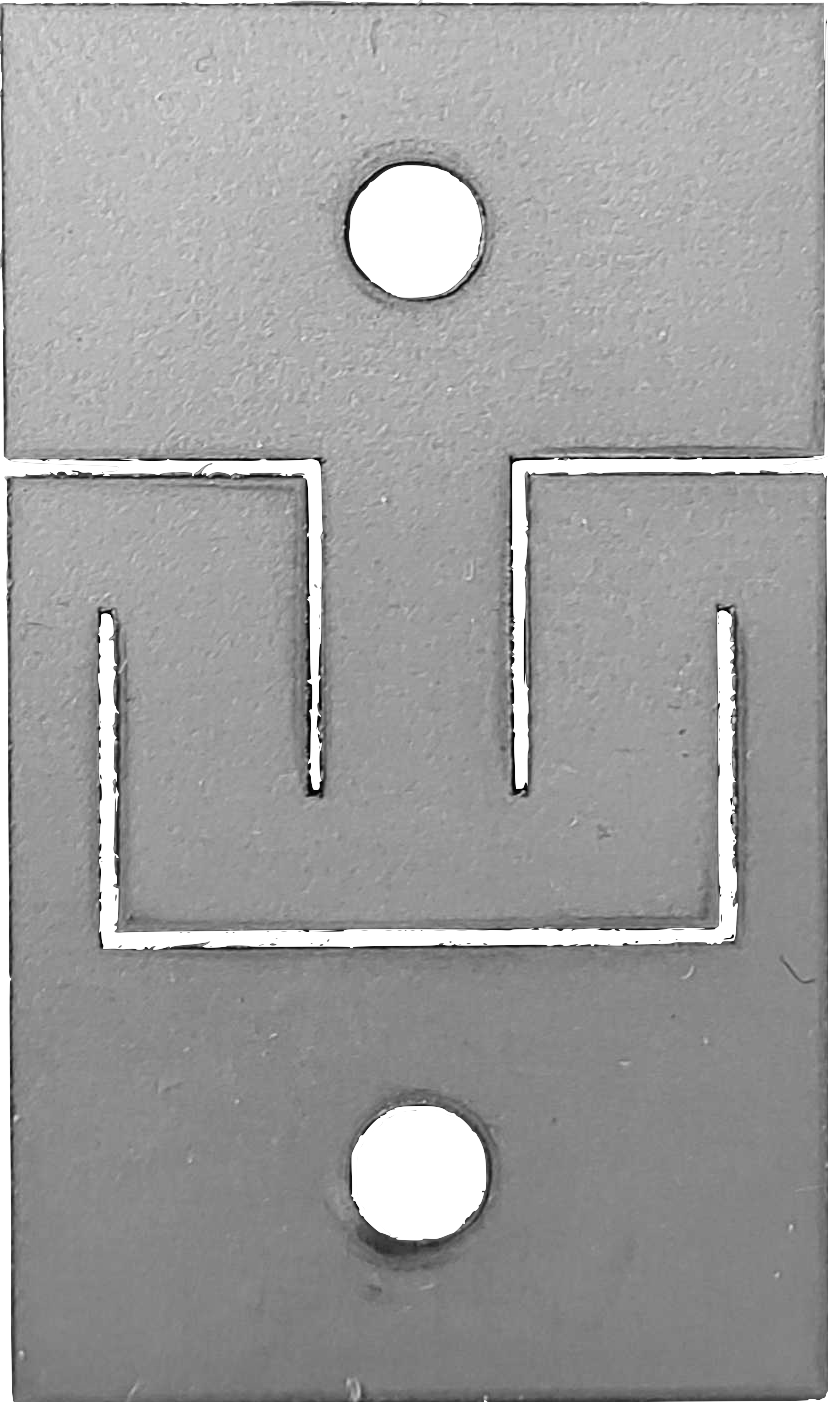
\includegraphics[height=0.5\textwidth]{images/chap5/sma-kiri-unit-grey.png}
         \caption{$\Omega$-Pattern}
         \label{fig:omega-pattern-simple}
     \end{subfigure}
     % \hfill
     \begin{subfigure}[b]{0.45\textwidth}
         \centering
         \includegraphics[height=0.5\textwidth]{images/chap5/sma-kiri-lotus-fixation.png}
         \caption{Lotus-Pattern}
         \label{fig:lotus-pattern-simple}
     \end{subfigure}
    \caption{The proposed kirigami patterns for the SMA actuator.}
    \label{fig:sma-kiri-patterns}
\end{figure}

% Talk about the FEM models of both patterns

% Talk about the analytical models of the omega pattern
\subsection{Implementation}
% Talk about the implementation of the two types of actuator
